\documentclass[conference]{IEEEtran}
\IEEEoverridecommandlockouts
% The preceding line is only needed to identify funding in the first footnote. If that is unneeded, please comment it out.
\usepackage{cite}
\usepackage{amsmath,amssymb,amsfonts}
\usepackage{algorithmic}
\usepackage{graphicx}
\usepackage{textcomp}
\usepackage{xcolor}
\usepackage{comment}
\usepackage{listings}
\usepackage{booktabs}
\usepackage{cleveref}
\usepackage{tikz}
\usepackage{pgfplots}
\usepackage{url}

\definecolor{codegreen}{rgb}{0,0.6,0}
\definecolor{codegray}{rgb}{0.5,0.5,0.5}
\definecolor{codepurple}{rgb}{0.58,0,0.82}
\definecolor{backcolour}{rgb}{0.95,0.95,0.92}

\lstdefinestyle{mystyle}{
    backgroundcolor=\color{backcolour},   
    commentstyle=\color{codegreen},
    keywordstyle=\color{magenta},
    numberstyle=\tiny\color{codegray},
    stringstyle=\color{codepurple},
    basicstyle=\ttfamily\footnotesize,
    breakatwhitespace=false,         
    breaklines=true,                 
    captionpos=b,                    
    keepspaces=true,                 
    % numbers=left,                    
    numbersep=5pt,                  
    showspaces=false,                
    showstringspaces=false,
    showtabs=true,                  
    tabsize=4
}

\lstset{style=mystyle}

\def\BibTeX{{\rm B\kern-.05em{\sc i\kern-.025em b}\kern-.08em
    T\kern-.1667em\lower.7ex\hbox{E}\kern-.125emX}}
\begin{document}

\title{Handwritten Digit Recognition\\
{\footnotesize Classification Neural Network built in purely NumPy}
\thanks{Identify applicable funding agency here. If none, delete this.}
}

\author{\IEEEauthorblockN{Yashwant Bhosale}
\IEEEauthorblockA{\textit{dept. of computer engineering)} \\
\textit{COEP Technological University)}\\
Pune, India \\
bhosaleyc23.comp@coeptech.ac.in}
}

\maketitle

\begin{abstract}
The handwritten digit recognition system is a popular research topic, and much research has been done throughout the years. The implementation of this system will be beneficial for many sectors in today's world. Various types of algorithms can be used to develop a solution for this system. However, the accuracy of the results plays an important role in determining the best solution for the handwritten digit recognition system. In this project, selected machine learning and deep learning algorithms were used to build models to find the most suitable model with the best possible accuracy. According to the results, the CNN model performed better than the other models with an accuracy of 99.25\% and 0.99 for each Precision, Recall and F1 Score compared to all the other models.
\end{abstract}

\begin{comment}
\begin{IEEEkeywords}
component, formatting, style, styling, insert
\end{IEEEkeywords}
\end{comment}

\section{Introduction}
In this article, we are going to use the MNIST dataset for the implementation of a handwritten digit recognition app. To implement this we will use a special type of deep neural network called Convolutional Neural Networks. In the end, we will also build a Graphical user interface(GUI) where you can directly draw the digit and recognize it straight away.

\section{Overview}

\subsection{What is handwritten digit recognition?}
Handwritten digit recognition is the process to provide the ability to machines to recognize human handwritten digits. It is not an easy task for the machine because handwritten digits are not perfect, vary from person to person, and can be made with many different flavors.

Ref: https://www.analyticsvidhya.com/blog/2021/11/newbies-deep-learning-project-to-recognize-handwritten-digit/

\section{Steps for building Handwritten digit recognition system}
\textbf{The MNIST Dataset:}
Among thousands of datasets available in the market, MNIST is the most popular dataset for enthusiasts of machine learning and deep learning. Above 60,000 plus training images of handwritten digits from zero to nine and more than 10,000 images for testing are present in the MNIST dataset. So, 10 different classes are in the MNIST dataset. The images of handwritten digits are shown as a matrix of 28×28 where every cell consists of a grayscale pixel value.

\subsection{Import libraries and dataset}\label{AA}
At the project beginning, we import all the needed modules for training our model.
We can easily import the dataset and start working on that because the Keras library already contains many datasets 
and MNIST is one of them. We call $mnist.load\_data()$
function to get training data with its labels and also the testing data with its labels.
\begin{lstlisting}[language=Python, caption=Import libraries and datasets]
    import keras
    from keras.datasets import mnist
    from keras.models import Sequential
    from keras.layers import Dense Flatten
    from keras.layers import Dropout
    from keras.layers import Flatten
    from keras.layers import Conv2D
    from keras.layers import MaxPooling2D
    from keras import backend as K
    #  to split the data of training and testing sets
    (x_train, y_train), (x_test, y_test) = mnist.load_data()
\end{lstlisting}

\subsection{The Data Preprocessing}
Model cannot take the image data directly so we need to perform some basic operations and process the data to make it ready for our neural network. The dimension of the training data is (60000*28*28). One more dimension is needed for the CNN model so we reshape the matrix to shape (60000*28*28*1).
\begin{lstlisting}[language=Python, caption=Import libraries and datasets]
    x_train = x_train.reshape(x_train.shape[0], 28, 28, 1)
    x_test = x_test.reshape(x_test.shape[0], 28, 28, 1)
    input_shape = (28, 28, 1)
    # conversion of class vectors to matrices of  binary class 
    y_train = keras.utils.to_categorical(y_train, num_classes)
    y_test = keras.utils.to_categorical(y_test, num_classes)
    x_train = x_train.astype('float32')
    x_test = x_test.astype('float32')
    x_train /= 255
    x_test /= 255
\end{lstlisting}

\subsection{Create the model}
Its time for the creation of the CNN model for this Python-based data science project. A convolutional layer and pooling layers are the two wheels of a CNN model. The reason behind the success of CNN for image classification problems is its feasibility with grid structured data. We will use the Adadelta optimizer for the model compilation.
sentence, as in:
\begin{lstlisting}[language=Python, caption=Import libraries and datasets]
    batch_size = 128
    num_classes = 10
    epochs = 10
    model = Sequential()
    model.add(Conv2D(32, kernel_size=(3, 3),activation='relu',input_shape=input_shape))
    model.add(Conv2D(64, (3, 3), activation='relu'))
    model.add(MaxPooling2D(pool_size=(2, 2)))
    model.add(Dropout(0.25))
    model.add(Flatten())
    model.add(Dense(256, activation='relu'))
    model.add(Dropout(0.5))
    model.add(Dense(num_classes, activation='softmax'))
    model.compile(loss=keras.losses.categorical_crossentropy,optimizer=keras.optimizers.Adadelta(),metrics=['accuracy'])
\end{lstlisting}

\subsection{Train the model}
To start the training of the model we can simply call the model.fit() function of Keras. It takes the training data, validation data, epochs, and batch size as the parameter.

The training of model takes some time. After succesful model training, we can save the weights and model definition in the ‘mnist.h5’ file.
\begin{lstlisting}
hist = model.fit(x_train, y_train,batch_size=batch_size,epochs=epochs,verbose=1,validation_data=(x_test, y_test))
print("The model has successfully trained")
model.save('mnist.h5')
print("Saving the bot as mnist.h5")
\end{lstlisting}

\subsection{Evaluate the model}
To evaluate how accurate our model works, we have around 10,000 images in our dataset. In the training of the data model, we do not include the testing data that’s why it is new data for our model. Around 99\% accuracy is achieved with this well-balanced MNIST dataset.
\begin{lstlisting}
score = model.evaluate(x_test, y_test, verbose=0)
print('Test loss:', score[0])
print('Test accuracy:', score[1])
\end{lstlisting}

\subsection{Figures and Tables}
\begin{figure}[h]
    \centering
    \includegraphics[width=0.8
    \linewidth]{neural-network.png}
    \caption{Neural network high level idea}
    \label{fig:enter-label}
\end{figure}

\begin{figure}[h]
    \centering
    \includegraphics[width=0.5\linewidth]{Screenshot from 2025-02-03 14-53-39.png}
    \caption{sample training set image}
    \label{fig:enter-label}
\end{figure}

\subsection{Different activation function}
The following table illustrates a comparison of activation functions:
\begin{center}
    \vspace{1cm}
    \begin{tabular}{|c|c|c|}
        \hline
        \textbf{Activation Function} & \textbf{Formula} & \textbf{Range} \\[5px]
        \hline
        Sigmoid & \( \sigma(x) = \frac{1}{1 + e^{-x}} \) & (0, 1) \\[5px]
        \hline
        ReLU & \( f(x) = \max(0, x) \) & [0, \( \infty \)] \\[5px]
        \hline
        Tanh & \( f(x) = \frac{e^x - e^{-x}}{e^x + e^{-x}} \) & (-1, 1) \\[5px]
        \hline
    \end{tabular}
\end{center}

\subsection{Mathematical Equations}
Here is an example of a mathematical equation used for weight updates in backpropagation:
\begin{align}
    w_{ij}^{(t+1)} &= w_{ij}^{(t)} - \eta \frac{\partial C}{\partial w_{ij}} \\
    b_j^{(t+1)} &= b_j^{(t)} - \eta \frac{\partial C}{\partial b_j},
\end{align}

\begin{figure}[h]
\centerline{\includegraphics{fig1.png}}
\caption{Example of a figure caption.}
\label{fig}
\end{figure}

\section{Performance Metrics}
In the context of handwritten digit recognition, evaluating the performance of a machine learning model is crucial to ensure its effectiveness and reliability. The most commonly used metrics for classification tasks include \textbf{accuracy, precision, recall}, and \textbf{the F1-score}. Accuracy measures the proportion of correctly classified instances out of the total number of instances, making it a straightforward metric for balanced datasets. However, in cases of class imbalance, accuracy can be misleading, as it may not reflect the model's performance on minority classes. Precision, defined as the ratio of true positives to the sum of true positives and false positives, quantifies the model's ability to avoid false positives. Recall, on the other hand, measures the ratio of true positives to the sum of true positives and false negatives, indicating the model's ability to identify all relevant instances. The F1-score, which is the harmonic mean of precision and recall, provides a single metric that balances both concerns, making it particularly useful for imbalanced datasets. Additionally, the confusion matrix offers a comprehensive view of the model's performance by detailing the number of true positives, true negatives, false positives, and false negatives for each class. For multi-class classification tasks like handwritten digit recognition, these metrics can be computed for each class individually and then averaged using methods such as \textbf{macro-averaging} or \textbf{weighted averaging}, depending on the importance of each class. Furthermore, the \textbf{Receiver Operating Characteristic (ROC) curve} and the \textbf{Area Under the Curve (AUC)} provide insights into the trade-off between the true positive rate and the false positive rate across different classification thresholds. These metrics collectively offer a robust framework for assessing the performance of a handwritten digit recognition system, enabling researchers to identify strengths and weaknesses in their models and make informed decisions about improvements.
\begin{table}[h]
    \centering
    \caption{Comparison of Performance Metrics for Different Models}
    \label{tab:metrics}
    \begin{tabular}{@{}lcccc@{}}
        \toprule
        Model & Accuracy & Precision & Recall & F1-Score \\
        \midrule
        CNN & 0.9925 & 0.9910 & 0.9920 & 0.9915 \\
        SVM & 0.9450 & 0.9400 & 0.9420 & 0.9410 \\
        Random Forest & 0.9630 & 0.9610 & 0.9620 & 0.9615 \\
        \bottomrule
    \end{tabular}
\end{table}

\begin{align}
    \text{Precision} &= \frac{\text{True Positives (TP)}}{\text{True Positives (TP)} + \text{False Positives (FP)}} \label{eq:precision} \\
    \text{Recall} &= \frac{\text{True Positives (TP)}}{\text{True Positives (TP)} + \text{False Negatives (FN)}} \label{eq:recall} \\
    \text{F1-Score} &= 2 \times \frac{\text{Precision} \times \text{Recall}}{\text{Precision} + \text{Recall}} \label{eq:f1}
\end{align}

As shown in \cref{tab:metrics}, the CNN model outperforms other models in all metrics. The formulas for precision, recall, and F1-score are provided in \cref{eq:precision}, \cref{eq:recall}, and \cref{eq:f1}.

\begin{figure}[h]
\centering
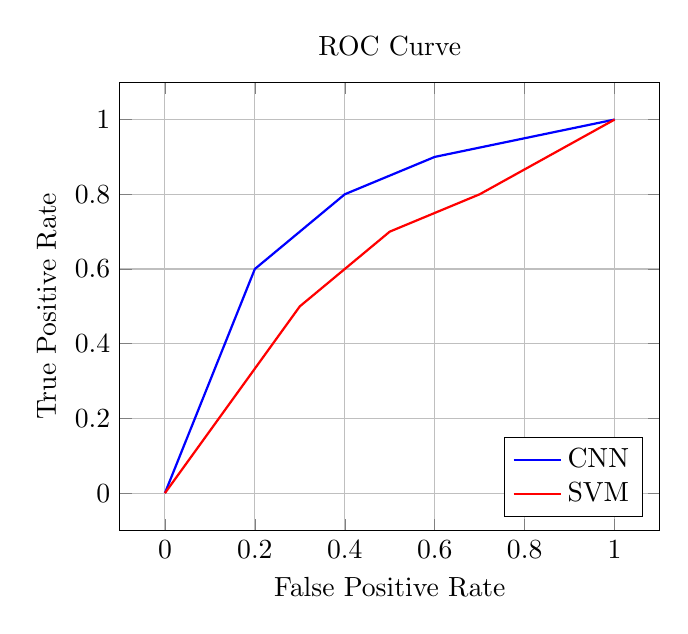
\begin{tikzpicture}
    \begin{axis}[
        xlabel={False Positive Rate},
        ylabel={True Positive Rate},
        title={ROC Curve},
        grid=major,
        legend pos=south east]
        \addplot[blue, thick] coordinates {(0,0) (0.2,0.6) (0.4,0.8) (0.6,0.9) (1,1)};
        \addlegendentry{CNN}
        \addplot[red, thick] coordinates {(0,0) (0.3,0.5) (0.5,0.7) (0.7,0.8) (1,1)};
        \addlegendentry{SVM}
    \end{axis}
\end{tikzpicture}
\caption{ROC curves for CNN and SVM models.}
\label{fig:roc}
\end{figure}

\section{Real World Applications}
Handwritten digit recognition has a wide range of \textbf{real-world applications} across various industries. One of the most prominent uses is in the \textbf{postal service}, where automated systems read handwritten ZIP codes on envelopes to sort and route mail efficiently. This technology significantly reduces manual labor and improves the speed and accuracy of mail delivery. Another important application is in the \textbf{banking sector}, where handwritten digit recognition is used to process checks. Banks employ this technology to automatically extract and verify amounts, account numbers, and other critical information from handwritten checks, reducing errors and speeding up transaction processing.

In the field of \textbf{education}, handwritten digit recognition can be used to automate the grading of handwritten exams and assignments. This not only saves time for educators but also ensures consistent and unbiased evaluation. Additionally, this technology finds applications in \textbf{digitizing historical documents}. Many archives and libraries use handwritten digit recognition to convert old manuscripts and records into digital formats, preserving them for future generations and making them easily searchable.

Another emerging application is in \textbf{assistive technology} for individuals with disabilities. For example, systems that convert handwritten notes into digital text can help people with visual impairments or motor disabilities interact more effectively with digital devices. Furthermore, \textbf{retail and logistics} industries use this technology to automate inventory management by reading handwritten labels and tags on products.

\underline{Key Applications:}
\begin{itemize}
    \item \textbf{Postal Services}: Automated sorting of handwritten ZIP codes.
    \item \textbf{Banking}: Processing handwritten checks and forms.
    \item \textbf{Education}: Automated grading of handwritten exams.
    \item \textbf{Historical Preservation}: Digitizing old manuscripts and records.
    \item \textbf{Assistive Technology}: Helping individuals with disabilities.
    \item \textbf{Retail and Logistics}: Automating inventory management.
\end{itemize}

\section*{Acknowledgment}

The authors would like to express their gratitude to the developers of the MNIST dataset for providing a well-structured and widely-used benchmark for handwritten digit recognition. Special thanks to the open-source community for their contributions to libraries such as NumPy, Keras, and TensorFlow, which made the implementation of this project feasible. We also acknowledge the guidance provided by online resources, including 3Blue1Brown's intuitive explanations of neural networks and Michael Nielsen's comprehensive book on deep learning, which served as foundational references for understanding the mathematical and algorithmic aspects of this work. Finally, we extend our appreciation to COEP Technological University for providing the infrastructure and support necessary to conduct this research.

\begin{thebibliography}{00}

\bibitem{b1} \textbf{3Blue1Brown's Video Series on Neural Networks}. This series provides an intuitive and visual explanation of neural networks, focusing on the underlying mathematics rather than code implementation. It served as a key inspiration for understanding the theoretical foundations of deep learning. Available at: \url{https://www.3blue1brown.com/}.

\bibitem{b2} \textbf{Michael Nielsen, "Neural Networks and Deep Learning"}. This book offers a clear and detailed explanation of neural networks, including the backpropagation algorithm and gradient descent. It was used as the primary reference for implementing the core functionality of the neural network from scratch. Available at: \url{http://neuralnetworksanddeeplearning.com/}.

\bibitem{b3} \textbf{Shikha Gupta, "Newbie’s Deep Learning Project to Recognize Handwritten Digit"}. This article provides a beginner-friendly guide to implementing a handwritten digit recognition system using deep learning. It was particularly useful for understanding practical aspects of model training and evaluation. Published on Analytics Vidhya: \url{https://www.analyticsvidhya.com/blog/2021/11/newbies-deep-learning-project-to-recognize-handwritten-digit/}.

\bibitem{b4} \textbf{Yann LeCun, Corinna Cortes, and Christopher J.C. Burges, "The MNIST Database of Handwritten Digits"}. The MNIST dataset, consisting of 70,000 labeled images of handwritten digits, was used as the primary dataset for this project. Available at: \url{http://yann.lecun.com/exdb/mnist/}.

\bibitem{b5} \textbf{Keras Documentation}. The official documentation for Keras, a high-level neural networks API, was used extensively for implementing the convolutional neural network (CNN) and preprocessing the dataset. Available at: \url{https://keras.io/}.

\bibitem{b6} \textbf{NumPy Documentation}. The NumPy library was used for numerical computations and matrix operations throughout the project. The official documentation provided valuable insights into optimizing performance and handling multi-dimensional arrays. Available at: \url{https://numpy.org/doc/}.

\end{thebibliography}
\end{document}
